
\documentclass[twoside]{article} % PREAMBLE

    \relax % Controls
        \newif\ifmarginprooflinks
        	\marginprooflinkstrue
        	% \marginprooflinksfalse

    \relax % Bibliography, etc
    	\usepackage[american]{babel}
    	\usepackage{csquotes}
    	\usepackage[backend=biber, style=authoryear]{biblatex}
    	\DeclareLanguageMapping{american}{american-apa}
    	% \usepackage[backend=biber,style=authoryear,hyperref=true]{biblatex}
    	\addbibresource{refs.bib}

    	\DeclareFieldFormat{citehyperref}{%
    	  \DeclareFieldAlias{bibhyperref}{noformat}% Avoid nested links
    	  \bibhyperref{#1}}

    	\DeclareFieldFormat{textcitehyperref}{%
    	  \DeclareFieldAlias{bibhyperref}{noformat}% Avoid nested links
    	  \bibhyperref{%
    	    #1%
    	    \ifbool{cbx:parens}
    	      {\bibcloseparen\global\boolfalse{cbx:parens}}
    	      {}}}

    	\savebibmacro{cite}
    	\savebibmacro{textcite}

    	\renewbibmacro*{cite}{%
    	  \printtext[citehyperref]{%
    	    \restorebibmacro{cite}%
    	    \usebibmacro{cite}}}

    	\renewbibmacro*{textcite}{%
    	  \ifboolexpr{
    	    ( not test {\iffieldundef{prenote}} and
    	      test {\ifnumequal{\value{citecount}}{1}} )
    	    or
    	    ( not test {\iffieldundef{postnote}} and
    	      test {\ifnumequal{\value{citecount}}{\value{citetotal}}} )
    	  }
    	    {\DeclareFieldAlias{textcitehyperref}{noformat}}
    	    {}%
    	  \printtext[textcitehyperref]{%
    	    \restorebibmacro{textcite}%
    	    \usebibmacro{textcite}}}

    	\DeclareCiteCommand{\brakcite}
    	  {\usebibmacro{prenote}}
    	  {\usebibmacro{citeindex}%
    	   \printtext[bibhyperref]{[\usebibmacro{cite}]}}
    	  {\multicitedelim}
    	  {\usebibmacro{postnote}}

    \relax % Standard Packages
        \usepackage[dvipsnames]{xcolor}
        % \usepackage[utf8]{inputenc}
        \usepackage{mathtools}
        \usepackage{amssymb}
    		\DeclareMathSymbol{\shortminus}{\mathbin}{AMSa}{"39}
        % \usepackage{parskip}
        % \usepackage{algorithm}
        \usepackage{bbm}
    	\usepackage{lmodern}
    	% \usepackage{times}
        \usepackage{faktor}
        % \usepackage{booktabs}
    	% \usepackage[margin=1in]{geometry}
        \usepackage{graphicx}
        \usepackage{scalerel}
        \usepackage{enumitem}
        \usepackage{nicefrac}\let\nf\nicefrac

        % \usepackage{color}
        %\usepackage{stmaryrd}
        \usepackage{hyperref} % Load before theorems...
            \hypersetup{colorlinks=true, linkcolor=blue!75!black, urlcolor=magenta, citecolor=green!50!black}

    \usepackage{tikz}
    	\usetikzlibrary{positioning,fit,calc, decorations, arrows, shapes, shapes.geometric}
    	\usetikzlibrary{cd}

    	%%%%%%%%%%%%
    	\tikzset{AmpRep/.style={ampersand replacement=\&}}
    	\tikzset{center base/.style={baseline={([yshift=-.8ex]current bounding box.center)}}}
    	\tikzset{paperfig/.style={center base,scale=0.9, every node/.style={transform shape}}}

    	% Node Stylings
    	\tikzset{dpadded/.style={rounded corners=2, inner sep=0.7em, draw, outer sep=0.3em, fill={black!50}, fill opacity=0.08, text opacity=1}}
    	\tikzset{dpad0/.style={outer sep=0.05em, inner sep=0.3em, draw=gray!75, rounded corners=4, fill=black!08, fill opacity=1, align=center}}
    	\tikzset{dpadinline/.style={outer sep=0.05em, inner sep=2.5pt, rounded corners=2.5pt, draw=gray!75, fill=black!08, fill opacity=1, align=center, font=\small}}

     	\tikzset{dpad/.style args={#1}{every matrix/.append style={nodes={dpadded, #1}}}}
    	\tikzset{light pad/.style={outer sep=0.2em, inner sep=0.5em, draw=gray!50}}

    	\tikzset{arr/.style={draw, ->, thick, shorten <=3pt, shorten >=3pt}}
    	\tikzset{arr0/.style={draw, ->, thick, shorten <=0pt, shorten >=0pt}}
    	\tikzset{arr1/.style={draw, ->, thick, shorten <=1pt, shorten >=1pt}}
    	\tikzset{arr2/.style={draw, ->, thick, shorten <=2pt, shorten >=2pt}}

    	\newcommand\cmergearr[5][]{
    		\draw[arr, #1, -] (#2) -- (#5) -- (#3);
    		\draw[arr, #1, shorten <=0] (#5) -- (#4);
    		}
    	\newcommand\mergearr[4][]{
    		\coordinate (center-#2#3#4) at (barycentric cs:#2=1,#3=1,#4=1.2);
    		\cmergearr[#1]{#2}{#3}{#4}{center-#2#3#4}
    		}
    	\newcommand\cunmergearr[5][]{
    		\draw[arr, #1, -, shorten >=0] (#2) -- (#5);
    		\draw[arr, #1, shorten <=0] (#5) -- (#3);
    		\draw[arr, #1, shorten <=0] (#5) -- (#4);
    		}
    	\newcommand\unmergearr[4][]{
    		\coordinate (center-#2#3#4) at (barycentric cs:#2=1.2,#3=1,#4=1);
    		\cunmergearr[#1]{#2}{#3}{#4}{center-#2#3#4}
    		}

    \usepackage{amsthm,thmtools} % Theorem Macros
    	\usepackage[noabbrev,nameinlink,capitalize]{cleveref}
        \theoremstyle{plain}
        \newtheorem{theorem}{Theorem}
    	\newtheorem{coro}{Corollary}[theorem]
        \newtheorem{prop}[theorem]{Proposition}
        \newtheorem{claim}{Claim}
        \newtheorem{remark}{Remark}
        \newtheorem{lemma}[theorem]{Lemma}
        \theoremstyle{definition}
        % \newtheorem{defn}{Definition}
        % \declaretheorem[name=Definition]{defn}
        \declaretheorem[name=Definition, qed=$\square$]{defn}
        \declaretheorem[name=Example, qed=$\triangle$]{example}

    	\crefname{defn}{Definition}{Definitions}
    	\crefname{prop}{Proposition}{Propositions}
        \crefname{issue}{Issue}{Issues}

    \relax %%%%%%%%% GENERAL MACROS %%%%%%%%
        \let\Horig\H
    	\let\H\relax
    	\DeclareMathOperator{\H}{\mathrm{H}} % Entropy
    	\DeclareMathOperator{\I}{\mathrm{I}} % Information
    	\DeclareMathOperator*{\Ex}{\mathbb{E}} % Expectation
    	\DeclareMathOperator*{\EX}{\scalebox{1.5}{$\mathbb{E}$}}

        \newcommand{\mat}[1]{\mathbf{#1}}
        \DeclarePairedDelimiterX{\infdivx}[2]{(}{)}{%
    		#1\;\delimsize\|\;#2%
    	}
    	\newcommand{\thickD}{I\mkern-8muD}
    	\newcommand{\kldiv}{\thickD\infdivx}
    	\newcommand{\tto}{\rightarrow\mathrel{\mspace{-15mu}}\rightarrow}

    	\newcommand{\datadist}[1]{\Pr\nolimits_{#1}}
    	% \newcommand{\datadist}[1]{p_\text{data}}

    	\makeatletter
    	\newcommand{\subalign}[1]{%
    	  \vcenter{%
    	    \Let@ \restore@math@cr \default@tag
    	    \baselineskip\fontdimen10 \scriptfont\tw@
    	    \advance\baselineskip\fontdimen12 \scriptfont\tw@
    	    \lineskip\thr@@\fontdimen8 \scriptfont\thr@@
    	    \lineskiplimit\lineskip
    	    \ialign{\hfil$\m@th\scriptstyle##$&$\m@th\scriptstyle{}##$\hfil\crcr
    	      #1\crcr
    	    }%
    	  }%
    	}
    	\makeatother
    	\newcommand\numberthis{\addtocounter{equation}{1}\tag{\theequation}}

    \relax %%%%%%%%%   PDG  MACROS   %%%%%%%%
    	\newcommand{\ssub}[1]{_{\!_{#1}\!}}
    	% \newcommand{\bp}[1][L]{\mat{p}_{\!_{#1}\!}}
    	% \newcommand{\bP}[1][L]{\mat{P}_{\!_{#1}\!}}
    	\newcommand{\bp}[1][L]{\mat{p}\ssub{#1}}
    	\newcommand{\bP}[1][L]{\mat{P}\ssub{#1}}
    	\newcommand{\V}{\mathcal V}
    	\newcommand{\N}{\mathcal N}
    	\newcommand{\Ed}{\mathcal E}

        \newcommand{\balpha}{\boldsymbol\alpha}
        \newcommand{\bbeta}{\boldsymbol\beta}

    	\DeclareMathAlphabet{\mathdcal}{U}{dutchcal}{m}{n}
    	\DeclareMathAlphabet{\mathbdcal}{U}{dutchcal}{b}{n}
    	\newcommand{\dg}[1]{\mathbdcal{#1}}
    	\newcommand{\PDGof}[1]{{\dg M}_{#1}}
    	\newcommand{\UPDGof}[1]{{\dg N}_{#1}}
    	\newcommand\VFE{\mathit{V\mkern-4mu F\mkern-4.5mu E}}

    	\newcommand\Inc{\mathit{Inc}}
    	\newcommand{\IDef}[1]{\mathit{IDef}_{\!#1}}
    	% \newcommand{\ed}[3]{%
    	% 	\mathchoice%
    	% 	{#2\overset{\smash{\mskip-5mu\raisebox{-3pt}{${#1}$}}}{\xrightarrow{\hphantom{\scriptstyle {#1}}}} #3} %display style
    	% 	{#2\overset{\smash{\mskip-5mu\raisebox{-3pt}{$\scriptstyle {#1}$}}}{\xrightarrow{\hphantom{\scriptstyle {#1}}}} #3}% text style
    	% 	{#2\overset{\smash{\mskip-5mu\raisebox{-3pt}{$\scriptscriptstyle {#1}$}}}{\xrightarrow{\hphantom{\scriptscriptstyle {#1}}}} #3} %script style
    	% 	{#2\overset{\smash{\mskip-5mu\raisebox{-3pt}{$\scriptscriptstyle {#1}$}}}{\xrightarrow{\hphantom{\scriptscriptstyle {#1}}}} #3}} %scriptscriptstyle
    	\newcommand{\ed}[3]{#2%
    	  \overset{\smash{\mskip-5mu\raisebox{-1pt}{$\scriptscriptstyle
    	        #1$}}}{\rightarrow} #3}

        \newcommand{\nhphantom}[2]{\sbox0{\kern-2%
    		\nulldelimiterspace$\left.\delimsize#1\vphantom{#2}\right.$}\hspace{-.97\wd0}}
    		% \nulldelimiterspace$\left.\delimsize#1%
    		% \vrule depth\dp#2 height \ht#2 width0pt\right.$}\hspace{-.97\wd0}}
    	\makeatletter
    	\newsavebox{\abcmycontentbox}
    	\newcommand\DeclareDoubleDelim[5]{
    	    \DeclarePairedDelimiterXPP{#1}[1]%
    			{% box must be saved in this pre code
    				\sbox{\abcmycontentbox}{\ensuremath{##1}}%
    			}{#2}{#5}{}%
    		    %%% Correct spacing, but doesn't work with externalize.
    			% {\nhphantom{#3}{##1}\hspace{1.2pt}\delimsize#3\mathopen{}##1\mathclose{}\delimsize#4\hspace{1.2pt}\nhphantom{#4}{##1}}
    			%%% Fast, but wrong spacing.
    			% {\nhphantom{#3}{~}\hspace{1.2pt}\delimsize#3\mathopen{}##1\mathclose{}\delimsize#4\hspace{1.2pt}\nhphantom{#4}{~}}
    			%%% with savebox.
    		    {%
    				\nhphantom{#3}{\usebox\abcmycontentbox}%
    				\hspace{1.2pt} \delimsize#3%
    				\mathopen{}\usebox{\abcmycontentbox}\mathclose{}%
    				\delimsize#4\hspace{1.2pt}%
    				\nhphantom{#4}{\usebox\abcmycontentbox}%
    			}%
    	}
    	\makeatother
    	\DeclareDoubleDelim
    		\SD\{\{\}\}
    	\DeclareDoubleDelim
    		\bbr[[]]
    	% \DeclareDoubleDelim
    	% 	\aar\langle\langle\rangle\rangle
    	\makeatletter
    	\newsavebox{\aar@content}
    	\newcommand\aar{\@ifstar\aar@one@star\aar@plain}
    	\newcommand\aar@one@star{\@ifstar\aar@resize{\aar@plain*}}
    	\newcommand\aar@resize[1]{\sbox{\aar@content}{#1}\scaleleftright[3.8ex]
    		{\Biggl\langle\!\!\!\!\Biggl\langle}{\usebox{\aar@content}}
    		{\Biggr\rangle\!\!\!\!\Biggr\rangle}}
    	\DeclareDoubleDelim
    		\aar@plain\langle\langle\rangle\rangle
    	\makeatother


    	% \DeclarePairedDelimiterX{\aar}[1]{\langle}{\rangle}
    	% 	{\nhphantom{\langle}{#1}\hspace{1.2pt}\delimsize\langle\mathopen{}#1\mathclose{}\delimsize\rangle\hspace{1.2pt}\nhphantom{\rangle}{#1}}

    \relax %%%%% restatables and links
    	% \usepackage{xstring} % for expandarg
    	\usepackage{xpatch}
    	\makeatletter
    	\xpatchcmd{\thmt@restatable}% Edit \thmt@restatable
    	   {\csname #2\@xa\endcsname\ifx\@nx#1\@nx\else[{#1}]\fi}% Replace this code
    	   % {\ifthmt@thisistheone\csname #2\@xa\endcsname\typeout{oiii[#1;#2\@xa;#3;\csname thmt@stored@#3\endcsname]}\ifx\@nx#1\@nx\else[#1]\fi\else\csname #2\@xa\endcsname\fi}% with this code
    	   {\ifthmt@thisistheone\csname #2\@xa\endcsname\ifx\@nx#1\@nx\else[{#1}]\fi
    	   \else\fi}
    	   {}{\typeout{FIRST PATCH TO THM RESTATE FAILED}} % execute on success/failure
    	\xpatchcmd{\thmt@restatable}% A second edit to \thmt@restatable
    	   {\csname end#2\endcsname}
    	   {\ifthmt@thisistheone\csname end#2\endcsname\else\fi}
    	   {}{\typeout{FAILED SECOND THMT RESTATE PATCH}}

    	% \def\onlyaftercolon#1:#2{#2}
    	\newcommand{\recall}[1]{\medskip\par\noindent{\bf \Cref{thmt@@#1}.} \begingroup\em \noindent
    	   \expandafter\csname#1\endcsname* \endgroup\par\smallskip}

       	\setlength\marginparwidth{1.55cm}
    	\newenvironment{linked}[3][]{%
    		\def\linkedproof{#3}%
    		\def\linkedtype{#2}%
    		% \reversemarginpar
    		% \marginpar{%
    		% \vspace{1.1em}
    		% % \hspace{2em}
    		% 	% \raggedleft
    		% 	\raggedright
    		% 	\hyperref[proof:\linkedproof]{%
    		% 	\color{blue!50!white}
    		% 	\scaleleftright{$\Big[$}{\,{\small\raggedleft\tt\begin{tabular}{@{}c@{}} proof of \\\linkedtype~\ref*{\linkedtype:\linkedproof}\end{tabular}}\,}{$\Big]$}}
    		% 	}%
            % \restatable[#1]{#2}{#2:#3}\label{#2:#3}%
    		\ifmarginprooflinks
    		\marginpar{%
    			% \vspace{-3em}% %% for bottom
    			\vspace{1.5em}
    			\centering%
    			\hyperref[proof:\linkedproof]{%
                % \hyperref[proof:#3]{
    			\color{blue!30!white}%
    			\scaleleftright{$\Big[$}{\,\mbox{\footnotesize\centering\tt\begin{tabular}{@{}c@{}}
    				% proof of \\\,\linkedtype~\ref*{\linkedtype:\linkedproof}
    				link to\\[-0.15em]
    				proof
    			\end{tabular}}\,}{$\Big]$}}~
    			}%
    		\fi
            \restatable[#1]{#2}{#2:#3}\label{#2:#3}%
            }%
    		{\endrestatable%
    		}
    	\makeatother
    		\newcounter{proofcntr}
    		\newenvironment{lproof}{\begin{proof}\refstepcounter{proofcntr}}{\end{proof}}

    		\usepackage{cancel}
    		\newcommand{\Cancel}[2][black]{{\color{#1}\cancel{\color{black}#2}}}

    		\usepackage{tcolorbox}
    		\tcbuselibrary{most}
    		\tcolorboxenvironment{lproof}{
    			% fonttitle=\bfseries,
    			% top=0.5em,
    			enhanced,
    			parbox=false,
    			boxrule=0pt,
    			frame hidden,
    			borderline west={4pt}{0pt}{blue!20!black!40!white},
    			% coltext={blue!20!black!60!white},
    			colback={blue!20!black!05!white},
    			sharp corners,
    			breakable,
    			% bottomsep at break=4cm,
    			% enlarge bottom at break by=-4cm,
    			% topsep at break=3cm,
    			% enlarge top at break by=-3cm
    		}
    		% \usepackage[framemethod=TikZ]{mdframed}
    		% \surroundwithmdframed[ % lproof
    		% 	   topline=false,
    		% 	   linewidth=3pt,
    		% 	   linecolor=gray!20!white,
    		% 	   rightline=false,
    		% 	   bottomline=false,
    		% 	   leftmargin=0pt,
    		% 	   % innerleftmargin=5pt,
    		% 	   skipabove=\medskipamount,
    		% 	   skipbelow=\medskipamount
    		% 	]{lproof}
    	%oli16: The extra space was because there was extra space in the paragraph, not
    	%because this length was too big. By breaking arrays, everything will be better.
    	\newcommand{\begthm}[3][]{\begin{#2}[{name=#1},restate=#3,label=#3]}

    \relax %TODOs and footnotes
        \newcommand{\TODO}[1][INCOMPLETE]{{\centering\Large\color{red}$\langle$~\texttt{#1}~$\rangle$\par}}
        \newcommand{\dfootnote}[1]{%
            \let\oldthefootnote=\thefootnote%
            % \addtocounter{footnote}{-1}%
    		\setcounter{footnote}{999}
            \renewcommand{\thefootnote}{\textdagger}%
            \footnote{#1}%
            \let\thefootnote=\oldthefootnote%
        }
    	\newcommand{\dfootnotemark}{
    		\footnotemark[999]
    	}

% \twocolumn
\setlength\parskip{1ex}
% \usepackage[margin=1.2in]{geometry}


\begin{document}
    \section*{PDG Multi-Divergences}
    We have already seen that
    \[
        \thickD^{\mathrm{P\mskip-2muD\mskip-1.5muG}}_{(r,s)}(p, q) :=
        \aar[\bigg]{\!\!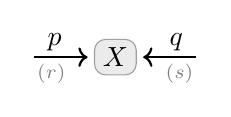
\begin{tikzpicture}[baseline = -0.75ex]
            \node[dpad0] (X) {$X$};
            \draw[arr2, <-] (X) --
                    % node[above] {$\overset{(\beta : r)}p$}
                    node[above, pos=0.6, inner sep=2pt, align=center] {$p$}
                    node[below, pos=0.65, inner sep=2pt, align=center]
                        % {$\scriptstyle{\color{gray}(\beta : r)}$}
                        {$\scriptstyle{\color{gray}(r)}$}
                ++(-1.1,0);
            \draw[arr2, <-] (X) --
                    % node[above,pos=0.5] {$\overset{(\beta : s)}q$}
                    node[above, pos=0.6, inner sep=2pt, align=center] {$q$}
                    node[below, pos=0.65, inner sep=2pt, align=center]
                        % {$\scriptstyle{\color{gray}(\beta : s)}$}
                        {$\scriptstyle{\color{gray}(s)}$}
                 ++(1.1, 0);
        \end{tikzpicture}\!\!}
        % = \thickD^{\mathrm{PDG}}_{(r,s)}(p, q)
        = - (r+s) \log  \sum_x \left(p(x)^{r}\vphantom{\Big|} q(x)^{s}\right)^{\frac{1}{r+s}}.
        % = - (r+s) \log \sum_x \! \sqrt[\leftroot{0}\uproot{2}r+s]{\vphantom{\big|}p(x)^{r} q(x)^{s}}
    % \qquad\text{where}\qquad \xi:= \beta_p+\beta_q
    \]
    But what if we have more divergences?
    \begin{prop}
        Consider a weighted collection of distributions $( p_i(X), \beta_i)_{i \in\mathcal I}$ on the same variable $X$, which form a PDG $\dg M$.  Then, writing $B := \sum_i \beta_i$, we have that
        \[
            \thickD^{\mathrm{P\mskip-2muD\mskip-1.5muG}}_{\bbeta}(\bp[\;]) := \qquad
            \aar{\dg M}
            = - B \log  \sum_x \prod_{i \in \mathcal I}
                p_i(x)^{\nicefrac{\beta_i}B} .
        \]
    \end{prop}


    The generalization to other values of $\gamma$ is also straightforward.
    \begin{prop}
        If $\dg M$ is the PDG comprising  $( p_i(X), \beta_i)_{i \in\mathcal I}$ and $B = \sum_i \beta_i$ as before, but now suppose each edge $i$ has some $\alpha_i$ and define $A = \sum_i\alpha_i$. Then,
        % \
        % \aar[\bigg]{\!\!\begin{tikzpicture}[baseline = -0.75ex]
        %     \node[dpad0] (X) {$X$};
        %     \draw[arr2, <-] (X) --
        %             % node[above] {$\overset{(\beta : r)}p$}
        %             node[above, pos=0.6, inner sep=2pt, align=center] {$p$}
        %             node[below, pos=0.65, inner sep=2pt, align=center]
        %                 % {$\scriptstyle{\color{gray}(\beta : r)}$}
        %                 {$\scriptstyle{\color{gray}(r)}$}
        %         ++(-1.1,0);
        %     \draw[arr2, <-] (X) --
        %             % node[above,pos=0.5] {$\overset{(\beta : s)}q$}
        %             node[above, pos=0.6, inner sep=2pt, align=center] {$q$}
        %             node[below, pos=0.65, inner sep=2pt, align=center]
        %                 % {$\scriptstyle{\color{gray}(\beta : s)}$}
        %                 {$\scriptstyle{\color{gray}(s)}$}
        %          ++(1.1, 0);
        % \end{tikzpicture}\!\!}_{\!\gamma}
        % \]
        \[
            % \thickD^{\mathrm{P\mskip-2muD\mskip-1.5muG}}_{\bbeta}(\bp[\;]) := \qquad
            \aar{\dg M}_\gamma
            = - (B + \gamma - \gamma A) \log  \sum_x \prod_{i \in \mathcal I}
                p_i(x)^{\nicefrac{\beta_i}{(B+\gamma-\gamma A)}}.
        \]
    \end{prop}

    % Some observations:
    \subsubsection*{Observations}
    \begin{enumerate}
        \item If $A = 1$, then the gamma-inconsistency is the same as before, and independent of $\gamma$ (since the causal picture exctly describes the randomness in the system, so $\IDef{}$ is the zero function).
        \item Now, suppose $A = 0$. Then $\gamma$ is just the coefficient on the entropy, and $\lim_{\gamma\to\infty} \aar{\dg M} = 0$, as the optimal distribution approaches uniform.

        \item As expected, if $B = \gamma A$, then
        \[
            \aar{\dg M}_\gamma = -  \gamma \log  \sum_x \prod_{i \in \mathcal I}
                p_i(x)^{\nicefrac{\beta_i}{\gamma}},
        \]
        so in particular, if $\gamma = 1$, then again the $\gamma$-inconsistency is independent of $\gamma$, so again $\aar{\dg M} = \aar{\dg M}_\gamma$.
    \end{enumerate}


    \section*{Starting instead with \texorpdfstring{$\chi^2$}{chi squared} divergences}

    \begin{prop}
        \[
        \thickD^{\mathrm{P\mskip-2muD\mskip-1.5muG.}\chi^2}_{(\beta,\zeta)}(p, q) :=
        \aar[\bigg]{\!\!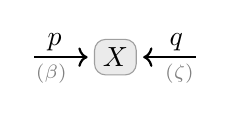
\begin{tikzpicture}[baseline = -0.75ex]
            \node[dpad0] (X) {$X$};
            \draw[arr2, <-] (X) --
                    % node[above] {$\overset{(\beta : r)}p$}
                    node[above, pos=0.6, inner sep=2pt, align=center] {$p$}
                    node[below, pos=0.65, inner sep=2pt, align=center]
                        % {$\scriptstyle{\color{gray}(\beta : r)}$}
                        {$\scriptstyle{\color{gray}(\beta)}$}
                ++(-1.1,0);
            \draw[arr2, <-] (X) --
                    % node[above,pos=0.5] {$\overset{(\beta : s)}q$}
                    node[above, pos=0.6, inner sep=2pt, align=center] {$q$}
                    node[below, pos=0.65, inner sep=2pt, align=center]
                        % {$\scriptstyle{\color{gray}(\beta : s)}$}
                        {$\scriptstyle{\color{gray}(\zeta)}$}
                 ++(1.1, 0);
        \end{tikzpicture}\!\!}^{\chi^2}
        = \frac{1}{\displaystyle \sum_x \frac{p(x)q(x)}{\zeta p(x) + \beta q(x)}} - (\beta+\zeta)
        \]
    \end{prop}


    \section*{Wasserstein Distances}

    Let $\Pi(p,q)$ be the set of couplings of $p$ and $q$, i.e.,

    \def\Tru{{\tt T}}
    \def\trut{{\tt t}}
    \def\truf{{\tt f}}

    \begin{prop}
        \[
            \aar**{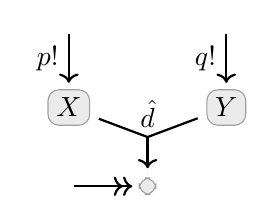
\begin{tikzpicture}[center base]
                \node[dpad0] (X) at (-1,0) {$X$};
                \node[dpad0] (Y) at (1,0) {$Y$};
                \node[dpad0] (T) at (0,-1) {$\Tru$};
                \draw[arr2, <<-] (T) to node[above]{$\trut$} +(-1,0);

                \draw[arr2, <-] (X) to
                    node[left]{$p!$}
                    +(0,1);
                \draw[arr2, <-] (Y) to
                    node[left]{$q!$}
                    +(0,1);

                \mergearr XYT
                \node[above=0pt of center-XYT] {$\hat d$};

            \end{tikzpicture}}
            = \inf_{\mu \in \Pi(p,q)} \Ex_{\mu} \Big[d(X,Y)\Big] = W_1(p,q),
        \]
    \end{prop}


    We also have:
    \begin{prop}
        \begin{align*}
            \aar**{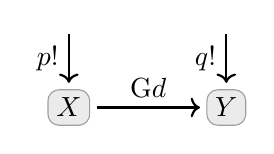
\begin{tikzpicture}[center base]
                \node[dpad0] (X) at (-1,0) {$X$};
                \node[dpad0] (Y) at (1,0) {$Y$};
                %
                \draw[arr2, <-] (X) to
                    node[left]{$p!$}
                    +(0,1);
                \draw[arr2, <-] (Y) to
                    node[left]{$q!$}
                    +(0,1);
                %
                \draw[arr2] (X) to
                    node[above]{$\mathrm G d$}
                    (Y);
                %
            \end{tikzpicture}}
            &=
            \inf_{\mu \in \Pi(p,q)} \Ex_{\mu} \Big[d(X,Y) + \log\sum_{y}\exp(-d(X,y))\Big] - \H(\mu) + \H(p) \\
            % &=
            % \inf_{\mu \in \Pi(p,q)} \Ex_{\mu} \Big[d(X,Y) + \mathrm{softmax}_y \big[ - d(X,y) \big] \Big] - \H(\mu) + \H(p)
        \end{align*}
    \end{prop}

    \begin{prop}
        \begin{align*}
            \lim_{t \to \infty} \frac1t \aar**{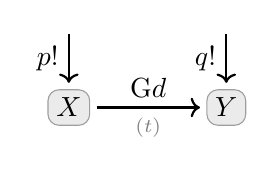
\begin{tikzpicture}[center base]
                \node[dpad0] (X) at (-1,0) {$X$};
                \node[dpad0] (Y) at (1,0) {$Y$};
                %
                \draw[arr2, <-] (X) to
                    node[left]{$p!$}
                    +(0,1);
                \draw[arr2, <-] (Y) to
                    node[left]{$q!$}
                    +(0,1);
                %
                \draw[arr2] (X) to
                    node[above]{$\mathrm G d$}
                    node[below]{${\color{gray}\scriptstyle(t)}$}
                    (Y);
                %
            \end{tikzpicture}}
            &=
            \inf_{\mu \in \Pi(p,q)} \Ex_{\mu} \Big[d(X,Y) \Big]
        \end{align*}
    \end{prop}
\end{document}
